\documentclass[12pt,a4paper,hidelinks]{article}

% General
\usepackage[utf8]{inputenc}
\usepackage{color}

% Graphics
\usepackage{graphicx}
\usepackage{epstopdf}
\usepackage{subcaption}
\usepackage{float}
\usepackage[export]{adjustbox}
\usepackage{wrapfig}
\usepackage{caption}

\captionsetup{
	justification = raggedright,
	singlelinecheck = false
}

% Page Layout
\usepackage{geometry}
\geometry{
	a4paper,
	left=25mm,
	top=35mm,
	right=25mm,
	bottom=30mm,
	%headsep=10mm,
	%head=0mm,
	foot=15mm,
	headheight=50mm,
}

% Paragraphs
%\setlength{\parindent}{0pt}
\usepackage{parskip}
\renewcommand{\baselinestretch}{1.2}
  
% Header / Footer
\usepackage{fancyhdr}
\usepackage{lastpage}

\pagestyle{fancy}
\renewcommand{\headrulewidth}{0pt}

\fancyhead[L]{
	\hspace{-0.61cm}
\includegraphics[width=9cm]{Resources/Document/fhnw-logo.pdf}
}
\fancyhead[R]{
	
\includegraphics[width=4.5cm]{Resources/Document/mse-logo.pdf}	
}

\cfoot{}
\fancyfoot[L]{
	Page \thepage\ of \pageref{LastPage}
}
\fancyfoot[R]{}

\fancypagestyle{firstpage}{	
	\fancyfoot[L]{}
	\fancyfoot[C]{IP-920bb}
	\fancyfoot[R]{}
}

% Todos
\usepackage{todonotes}
\usepackage{xcolor}
\newcommand\mytodo[1]{\textcolor{red}{TODO: #1}}

% Debug
\usepackage{layout}

% Bibliography
\bibliographystyle{IEEEtran}

% References
\usepackage{hyperref}
\usepackage{nameref}
\newcommand\myref[1]{(see \ref{#1} \nameref{#1})}

% Foot notes
\usepackage[bottom]{footmisc}

% Glossary
% see https://www.dickimaw-books.com/gallery/glossaries-styles/#long
\usepackage[nogroupskip,toc,nonumberlist]{glossaries}
%\usepackage[style=long2colheader]{glossaries-extra}

%\renewcommand*\pagelistname{Pages}
%\setlength{\LTleft}{-5pt}
%\setlength{\glsdescwidth}{8.5cm}

\loadglsentries{Glossary.tex}
\makeglossaries

% Footnotes
\makeatletter
\renewcommand\@makefntext[1]{\leftskip=2em\hskip-2em\@makefnmark#1}
\def\footnoterule{\kern-3mm\kern-3\p@
  \hrule \@width 2in \kern 2.6\p@
  \kern 2mm}
\makeatother

% Drawing
\usepackage{tikz}
\definecolor{fhnw_yellow}{rgb}{0.992, 0.905, 0.054}
\definecolor{my_orange}{rgb}{0.988, 0.792, 0.274}
\definecolor{my_red}{rgb}{0.847, 0.278, 0.25}
\definecolor{my_green}{rgb}{0.631, 0.756, 0.506}

% Tables
\usepackage{booktabs}
\usepackage{tabu}
\usepackage{tabularx}
\usepackage{colortbl}

% Table of contents
\usepackage{tocloft}
\usepackage[nottoc]{tocbibind}

\setcounter{tocdepth}{2}

\renewcommand{\cftpartfont}{\normalfont} % make parts look like sections in TOC
\renewcommand{\cftpartpagefont}{\normalfont}

\setlength{\cftbeforepartskip}{0pt} % remove spaces before and after chapters
\setlength{\cftfigindent}{0pt} % remove indentation from figures in lof
\setlength{\cfttabindent}{0pt} % remove indentation from tables in lot

\tocloftpagestyle{fancy}

% Code highlighting
\usepackage[newfloat]{minted}
\usepackage{xpatch}

\newenvironment{code}{\captionsetup{type=listing}}{}
\SetupFloatingEnvironment{listing}{name=Source Code}

\usemintedstyle{tango}

\renewcommand{\theFancyVerbLine}{\textcolor[rgb]{0.6,0.6,0.6}{\arabic{FancyVerbLine}}}

\xpatchcmd{\mintinline}{\begingroup}{\begingroup\let\itshape\relax}{}{}
\xpatchcmd{\minted}{\VerbatimEnvironment}{\VerbatimEnvironment\let\itshape\relax}{}{}


% Document
\begin{document}
	%\layout % Debug page layout
	\title{
		\vspace{50mm}
		\Huge{latex thesis template title}\\
	}
	\author{
		\\\\\normalsize{Author}\\
		Markus Mächler\\~\\
		\normalsize{Supervisor}\\
		Prof. Dr. Lorem Ipsum\\~\\
		\normalsize{University}\\
		Institute of Mobile and Distributed Systems\\
		FHNW\\~\\
	}
	\date{\normalsize{January 1, 1970}}
	\maketitle	
	\thispagestyle{firstpage} % Remove numbering in footer
	
	\section*{Abstract}
\label{sec:abstract}

Despite the fact that an abstract is quite brief, it must do almost as much work as the multi-page paper that follows it.
In a computer architecture paper, this means that it should in most cases include the following sections.
Each section is typically a single sentence, although there is room for creativity. In particular, the parts may be merged or spread among a set of sentences.
Use the following as a checklist for your next abstract:

\textit{Motivation:}
Why do we care about the problem and the results? If the problem isn't obviously "interesting" it might be better to put motivation first;
but if your work is incremental progress on a problem that is widely recognized as important, then it is probably better to put the problem statement first to indicate which piece of the larger problem you are breaking off to work on.
This section should include the importance of your work, the difficulty of the area, and the impact it might have if successful.

\textit{Problem statement:}
What problem are you trying to solve? What is the scope of your work (a generalized approach, or for a specific situation)?
Be careful not to use too much jargon. In some cases it is appropriate to put the problem statement before the motivation, but usually this only works if most readers already understand why the problem is important.

\textit{Approach:}
How did you go about solving or making progress on the problem?
Did you use simulation, analytic models, prototype construction, or analysis of field data for an actual product? What was the extent of your work (did you look at one application program or a hundred programs in twenty different programming languages?)
What important variables did you control, ignore, or measure?

\textit{Results:}
What's the answer? Specifically, most good computer architecture papers conclude that something is so many percent faster, cheaper, smaller, or otherwise better than something else.
Put the result there, in numbers. Avoid vague, hand-waving results such as "very", "small", or "significant."
If you must be vague, you are only given license to do so when you can talk about orders-of-magnitude improvement.
There is a tension here in that you should not provide numbers that can be easily misinterpreted, but on the other hand you don't have room for all the caveats.

\textit{Conclusions:}
What are the implications of your answer? Is it going to change the world (unlikely), be a significant "win", be a nice hack, or simply serve as a road sign indicating that this path is a waste of time (all of the previous results are useful).
Are your results general, potentially generalizable, or specific to a particular case? \cite{how_to_write_an_abstract_1997}

	\tableofcontents
	\section{Introduction}
\label{sec:introduction}

\subsection{Initial situation}
\label{sec:introduction:initial_situation}

Lorem ipsum dolor sit amet, consetetur sadipscing elitr, sed diam nonumy eirmod tempor invidunt ut labore et dolore magna aliquyam erat, sed diam voluptua. At vero eos et accusam et justo duo dolores et ea rebum. Stet clita kasd gubergren, no sea takimata sanctus est Lorem ipsum dolor sit amet. Lorem ipsum dolor sit amet, consetetur sadipscing elitr, sed diam nonumy eirmod tempor invidunt ut labore et dolore magna aliquyam erat, sed diam voluptua. At vero eos et accusam et justo duo dolores et ea rebum. Stet clita kasd gubergren, no sea takimata sanctus est Lorem ipsum dolor sit amet.

\subsection{Problem}
\label{sec:introduction:problem}

Lorem ipsum dolor sit amet, consetetur sadipscing elitr, sed diam nonumy eirmod tempor invidunt ut labore et dolore magna aliquyam erat, sed diam voluptua. At vero eos et accusam et justo duo dolores et ea rebum. Stet clita kasd gubergren, no sea takimata sanctus est Lorem ipsum dolor sit amet. Lorem ipsum dolor sit amet, consetetur sadipscing elitr, sed diam nonumy eirmod tempor invidunt.

\subsection{Goal}
\label{sec:introduction:goal}

Lorem ipsum dolor sit amet, consetetur sadipscing elitr, sed diam nonumy eirmod tempor invidunt ut labore et dolore magna aliquyam erat, sed diam voluptua. At vero eos et accusam et justo duo dolores et ea rebum. Stet clita kasd gubergren, no sea takimata sanctus est Lorem ipsum dolor sit amet. Lorem ipsum dolor sit amet, consetetur sadipscing elitr, sed diam nonumy eirmod tempor invidunt ut labore et dolore magna aliquyam erat, sed diam voluptua. At vero eos et accusam et justo duo dolores et ea rebum.

\subsection{Structure}
\label{sec:introduction:structure}

Lorem ipsum dolor sit amet, consetetur sadipscing elitr \ref{sec:typography}. At vero eos et accusam et justo duo dolores et ea rebum \ref{sec:images}. Stet clita kasd gubergren, no sea takimata sanctus est Lorem ipsum dolor sit amet \ref{sec:formulas}.

	\section{Typography}
\label{sec:typography}

\subsection{Subsection headline}
\label{sec:typography:subsection}

\subsubsection{Subsubsection headline}
\label{sec:typography:subsection:subsubsection}

\gls{Lorem ipsum} dolor sit amet, consetetur sadipscing elitr, sed diam nonumy eirmod tempor invidunt ut labore et dolore magna aliquyam erat, sed diam voluptua. At vero eos et accusam et justo duo dolores et ea rebum. Stet clita kasd gubergren, no sea takimata sanctus est Lorem ipsum dolor sit amet. Lorem ipsum dolor sit amet, consetetur sadipscing elitr, sed diam nonumy eirmod tempor invidunt ut labore et dolore magna aliquyam erat, sed diam voluptua. At vero eos et accusam et justo duo dolores et ea rebum. Stet clita kasd gubergren, no sea takimata sanctus est Lorem ipsum dolor sit amet.\footnote{This is a footnote: \url{https://loremipsum.de/}, accessed on 01.01.1970}

\textit{Italic lorem text}

\textbf{Bold lorem text}

This is a URL \url{https://github.com/maechler/latex-thesis-template}

\mytodo{This is a TODO note to improve this and that.}

\subsection{Lists}
\label{sec:typography:lists}

\subsubsection{Unorderered list}
\label{sec:typography:lists:unordered}

\begin{itemize}
	\item[$-$] \textbf{Lorem ipsum:} dolor sit amet, consetetur sadipscing elitr, sed diam nonumy eirmod tempor invidunt ut labore. Stet clita kasd gubergren, no sea takimata sanctus est Lorem ipsum dolor sit amet.
	
	\item[$-$] \textbf{Lorem:} ipsum dolor sit amet, consetetur sadipscing elitr, sed diam nonumy eirmod tempor invidunt ut labore.
\end{itemize}

\subsubsection{Orderered list}
\label{sec:typography:lists:ordered}

\begin{enumerate}
  \item First point
  \item Second point
\end{enumerate}

Lorem ipsum table \ref{table:typography:interesting_table} dolor sit amet, consetetur sadipscing elitr, sed diam nonumy eirmod tempor invidunt ut labore et dolore magna aliquyam erat, sed diam voluptua.

\subsection{Tables}
\label{sec:typography:tables}

\begin{table}[ht]
	\begingroup
		\abovetabulinesep=2mm
		\belowtabulinesep=2mm

		\begin{tabu} to \textwidth {X[2]X[1]X[1]}
			\textbf{Headline 1} & \textbf{Headline 2} & \textbf{Headline 3} \\
			\toprule
			Data value 1 & 21.1 & 63.5 \\
			Data value 2 & 11.7 & 49.8 \\
			Data value 3 & 11.2 & 77.6 \\
			\bottomrule 
		\end{tabu}
	\endgroup
	\caption{An interesting table}
	\label{table:typography:interesting_table}
\end{table}

\subsection{Source code}
\label{sec:typography:source_code}

Lorem ipsum dolor sit amet, consetetur sadipscing elitr, sed diam nonumy eirmod tempor invidunt ut labore et dolore magna aliquyam erat, sed diam voluptua.

\vspace{5mm}

\begin{code}
\begin{minted}[xleftmargin=0.8cm,linenos]{python}
import argparse


def say_hello(name: str) -> None:
    print("Hello " + str(name)) # Say hello


if __name__ == '__main__':
    parser = argparse.ArgumentParser()

    parser.add_argument('-n', '--name', type=str, required=True)
    
    args = parser.parse_args()

    say_hello(args.name)
\end{minted}

\caption{hello.py: Says hello to people that know how to handle it}
\label{list:hello}
\end{code}

	\section{Images}
\label{sec:images}

\subsection{Text wrapping}
\label{sec:images:text_wrapping}

\begin{wrapfigure}{r}{0.5\textwidth}
  \begin{center}
    \vspace{-1\intextsep}
    \hspace*{-.5\columnsep}
    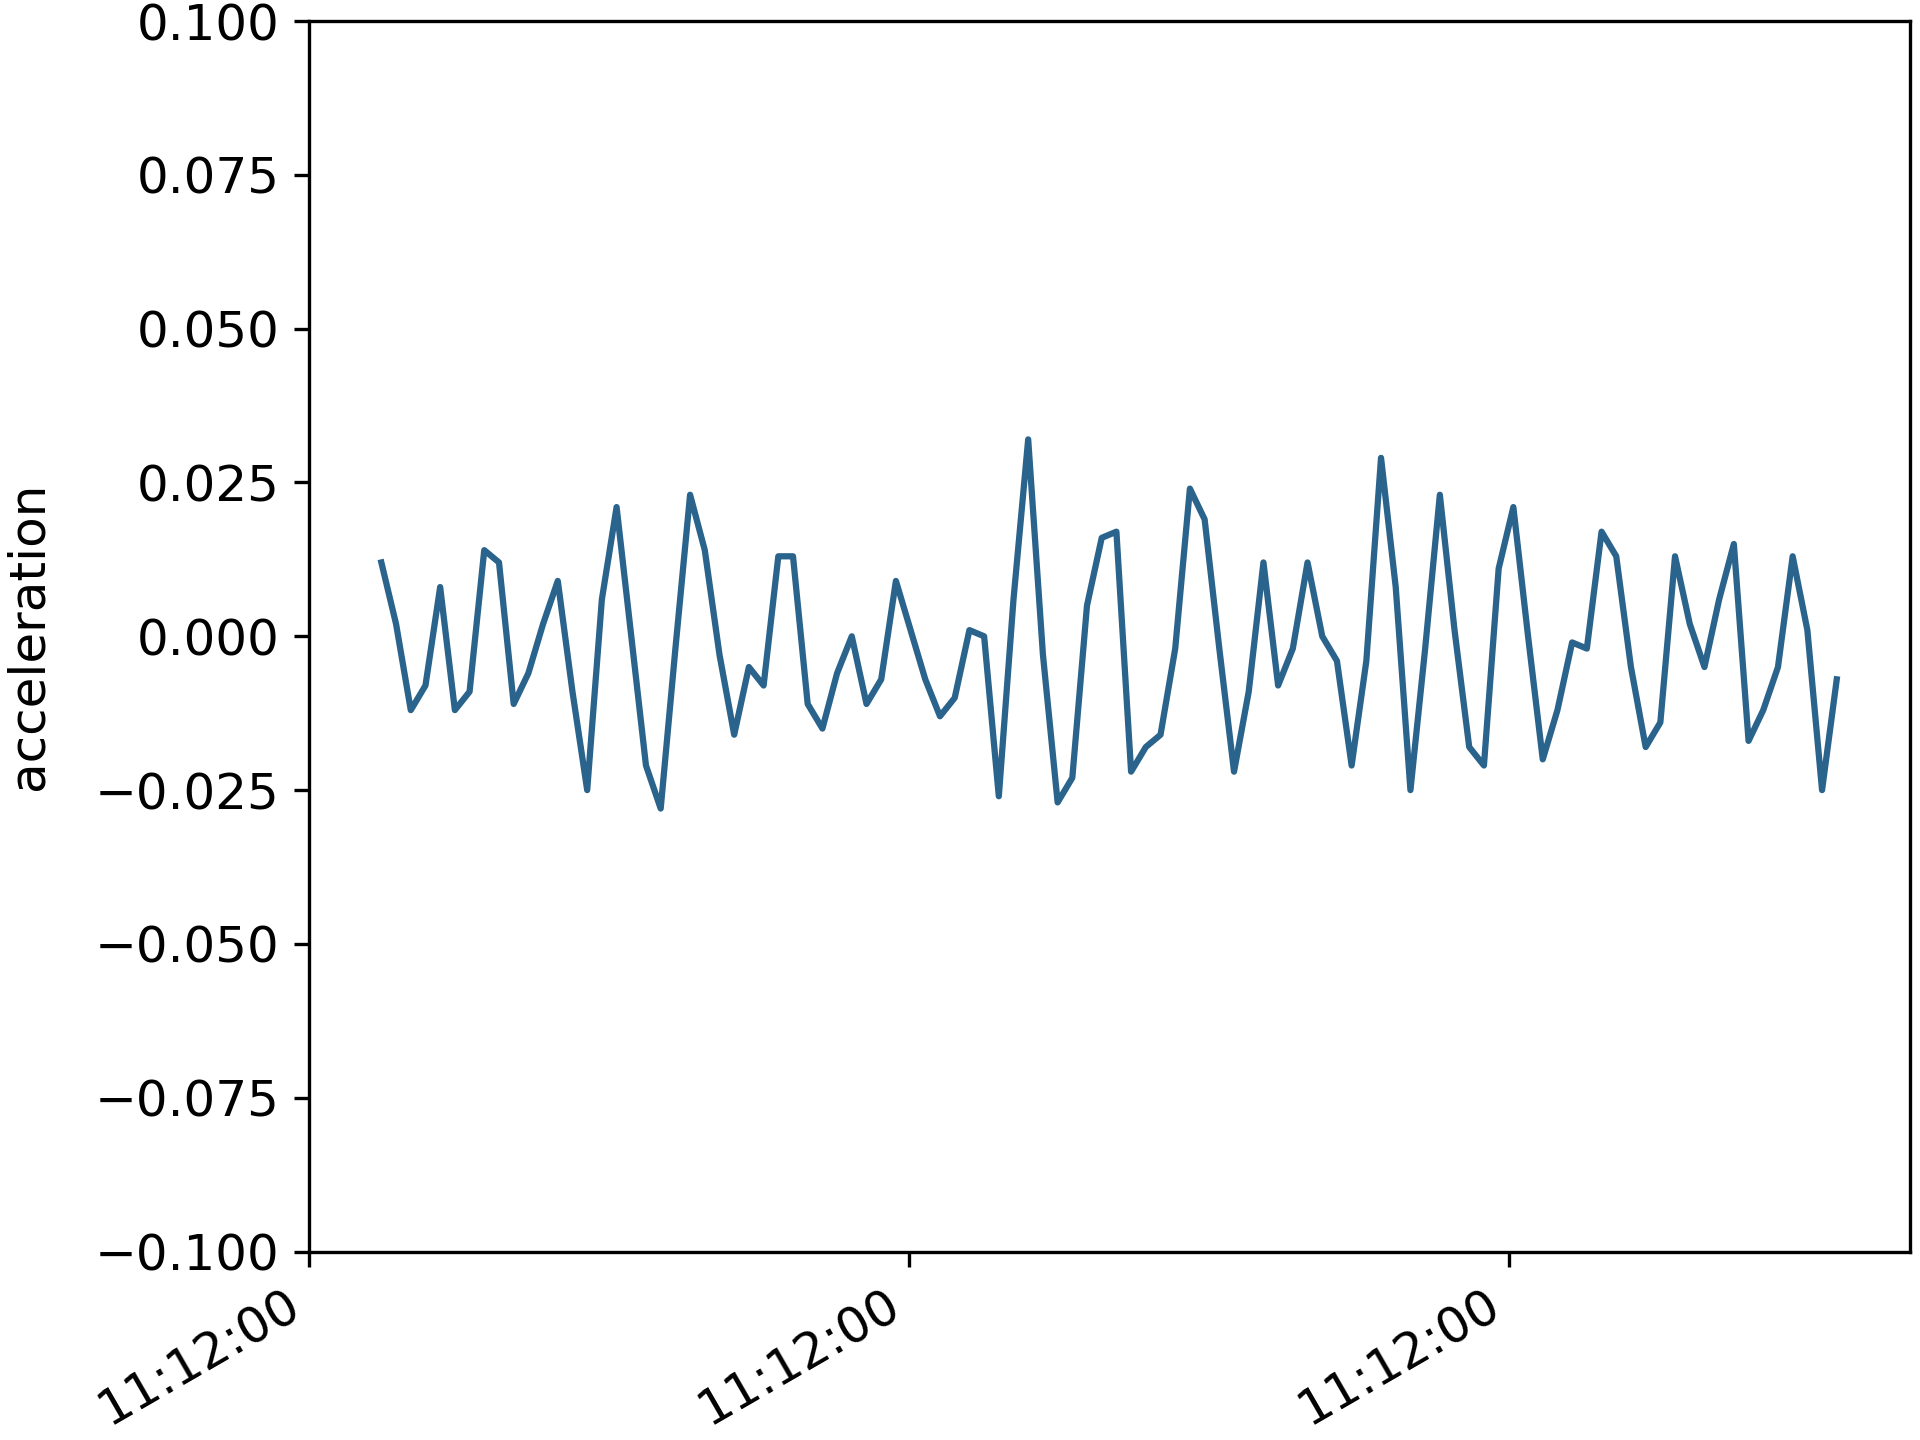
\includegraphics[width=0.5\textwidth]{Resources/Images/Bearing/bearing_acceleration.png}
  \end{center}
  \caption{Bearing acceleration of something}
  \label{fig:images:acceleration}
\end{wrapfigure}

As shown in figure \ref{fig:images:acceleration} lorem ipsum dolor sit amet, consetetur sadipscing elitr, sed diam nonumy eirmod tempor invidunt ut labore et dolore magna aliquyam erat, sed diam voluptua.
At vero eos et accusam et justo duo dolores et ea rebum. Stet clita kasd gubergren, no sea takimata sanctus est Lorem ipsum dolor sit amet.
Lorem ipsum dolor sit amet, consetetur sadipscing elitr, sed diam nonumy eirmod tempor invidunt ut labore et dolore magna aliquyam erat, sed diam voluptua. At vero eos et accusam et justo duo dolores et ea rebum.
Stet clita kasd gubergren, no sea takimata sanctus est Lorem ipsum dolor sit amet. Lorem ipsum dolor sit amet, consetetur sadipscing elitr, sed diam nonumy eirmod tempor invidunt ut labore et dolore magna aliquyam erat, sed diam voluptua.
At vero eos et accusam et justo duo dolores et ea rebum. \cite{example_xy}

\subsection{Centred image}
\label{sec:images:centred_image}

\begin{figure}[H]
	\begin{center}
		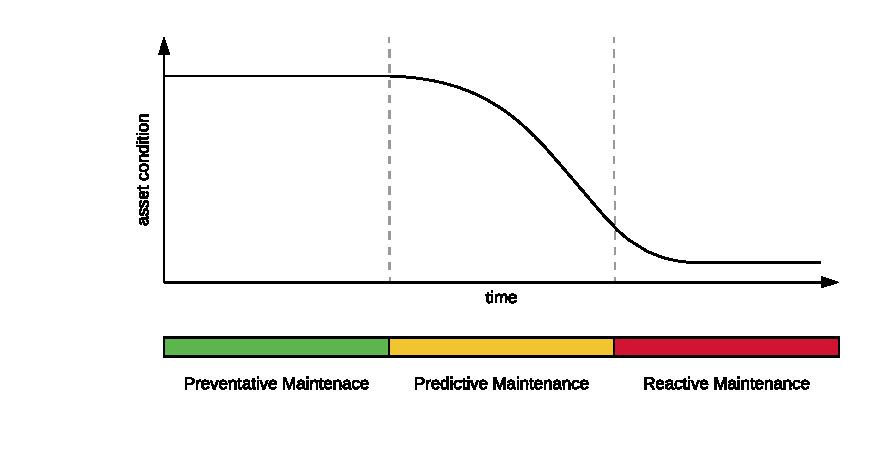
\includegraphics[width=.9\textwidth, clip, trim=1cm 1cm 0.5cm 0.5cm]{Resources/Images/Maintenance/maintenance_types.pdf}
	\end{center}
	\caption{Different types of maintenance}
	\label{fig:images:maintenance_types}
\end{figure}

\subsection{Two images side by side}
\label{sec:images:two_images}

\begin{figure}[H]
	\begin{minipage}{.475\textwidth}
		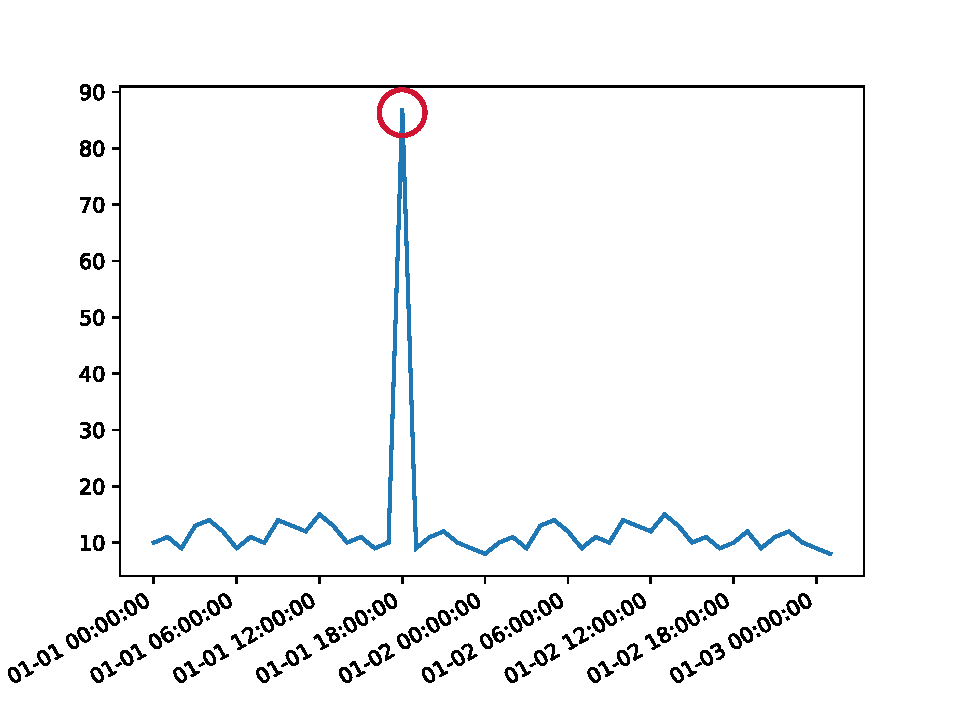
\includegraphics[width=\textwidth, clip, trim=0cm 0.5cm 1cm 1cm]{Resources/Images/Anomalies/point_anomaly.pdf}
		\caption{Point anomaly}
		\label{fig:images:point_anomaly}
	\end{minipage}
	\hspace{0.05\textwidth}
	\begin{minipage}{.475\textwidth}
		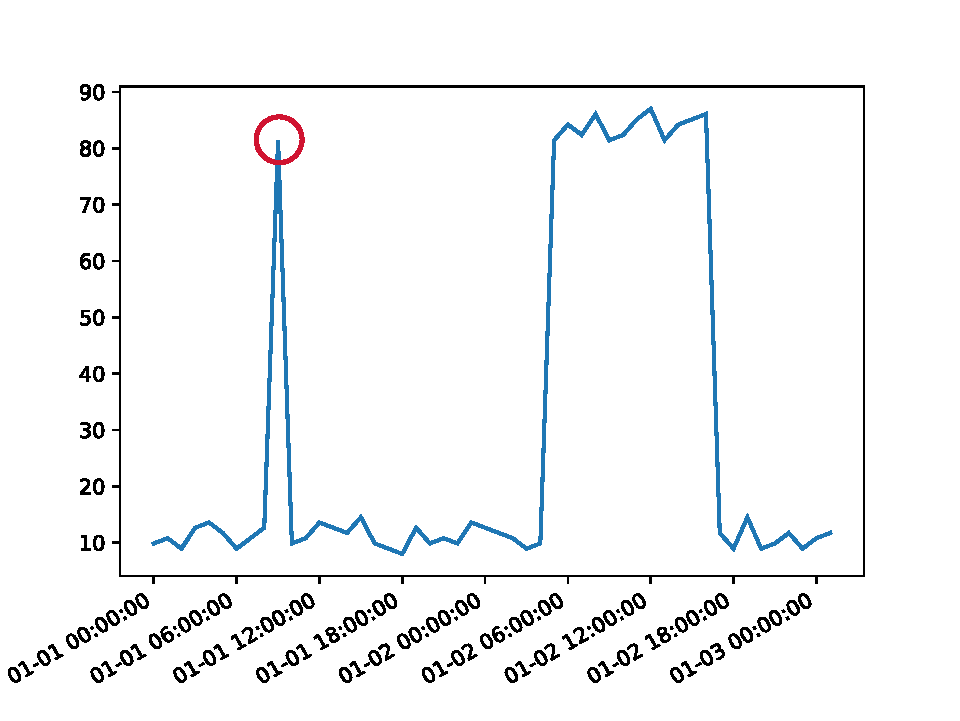
\includegraphics[width=\textwidth, clip, trim=0cm 0.5cm 1cm 1cm]{Resources/Images/Anomalies/contextual_anomaly.pdf}
		\caption{Contextual anomaly}
		\label{fig:images:contextual_anomaly}
	\end{minipage}
\end{figure}


\subsection{Three images side by side (one caption)}
\label{sec:images:three_images}

\begin{figure}[H]
	\begin{tabu} to \textwidth {XXX}
   	\centering\textbf{\footnotesize{Lorem ipsum}} & \centering\textbf{\footnotesize{Dolor sit}} & \centering\textbf{\footnotesize{Amet}} \\
	\end{tabu}
	\begin{minipage}{.325\textwidth}
		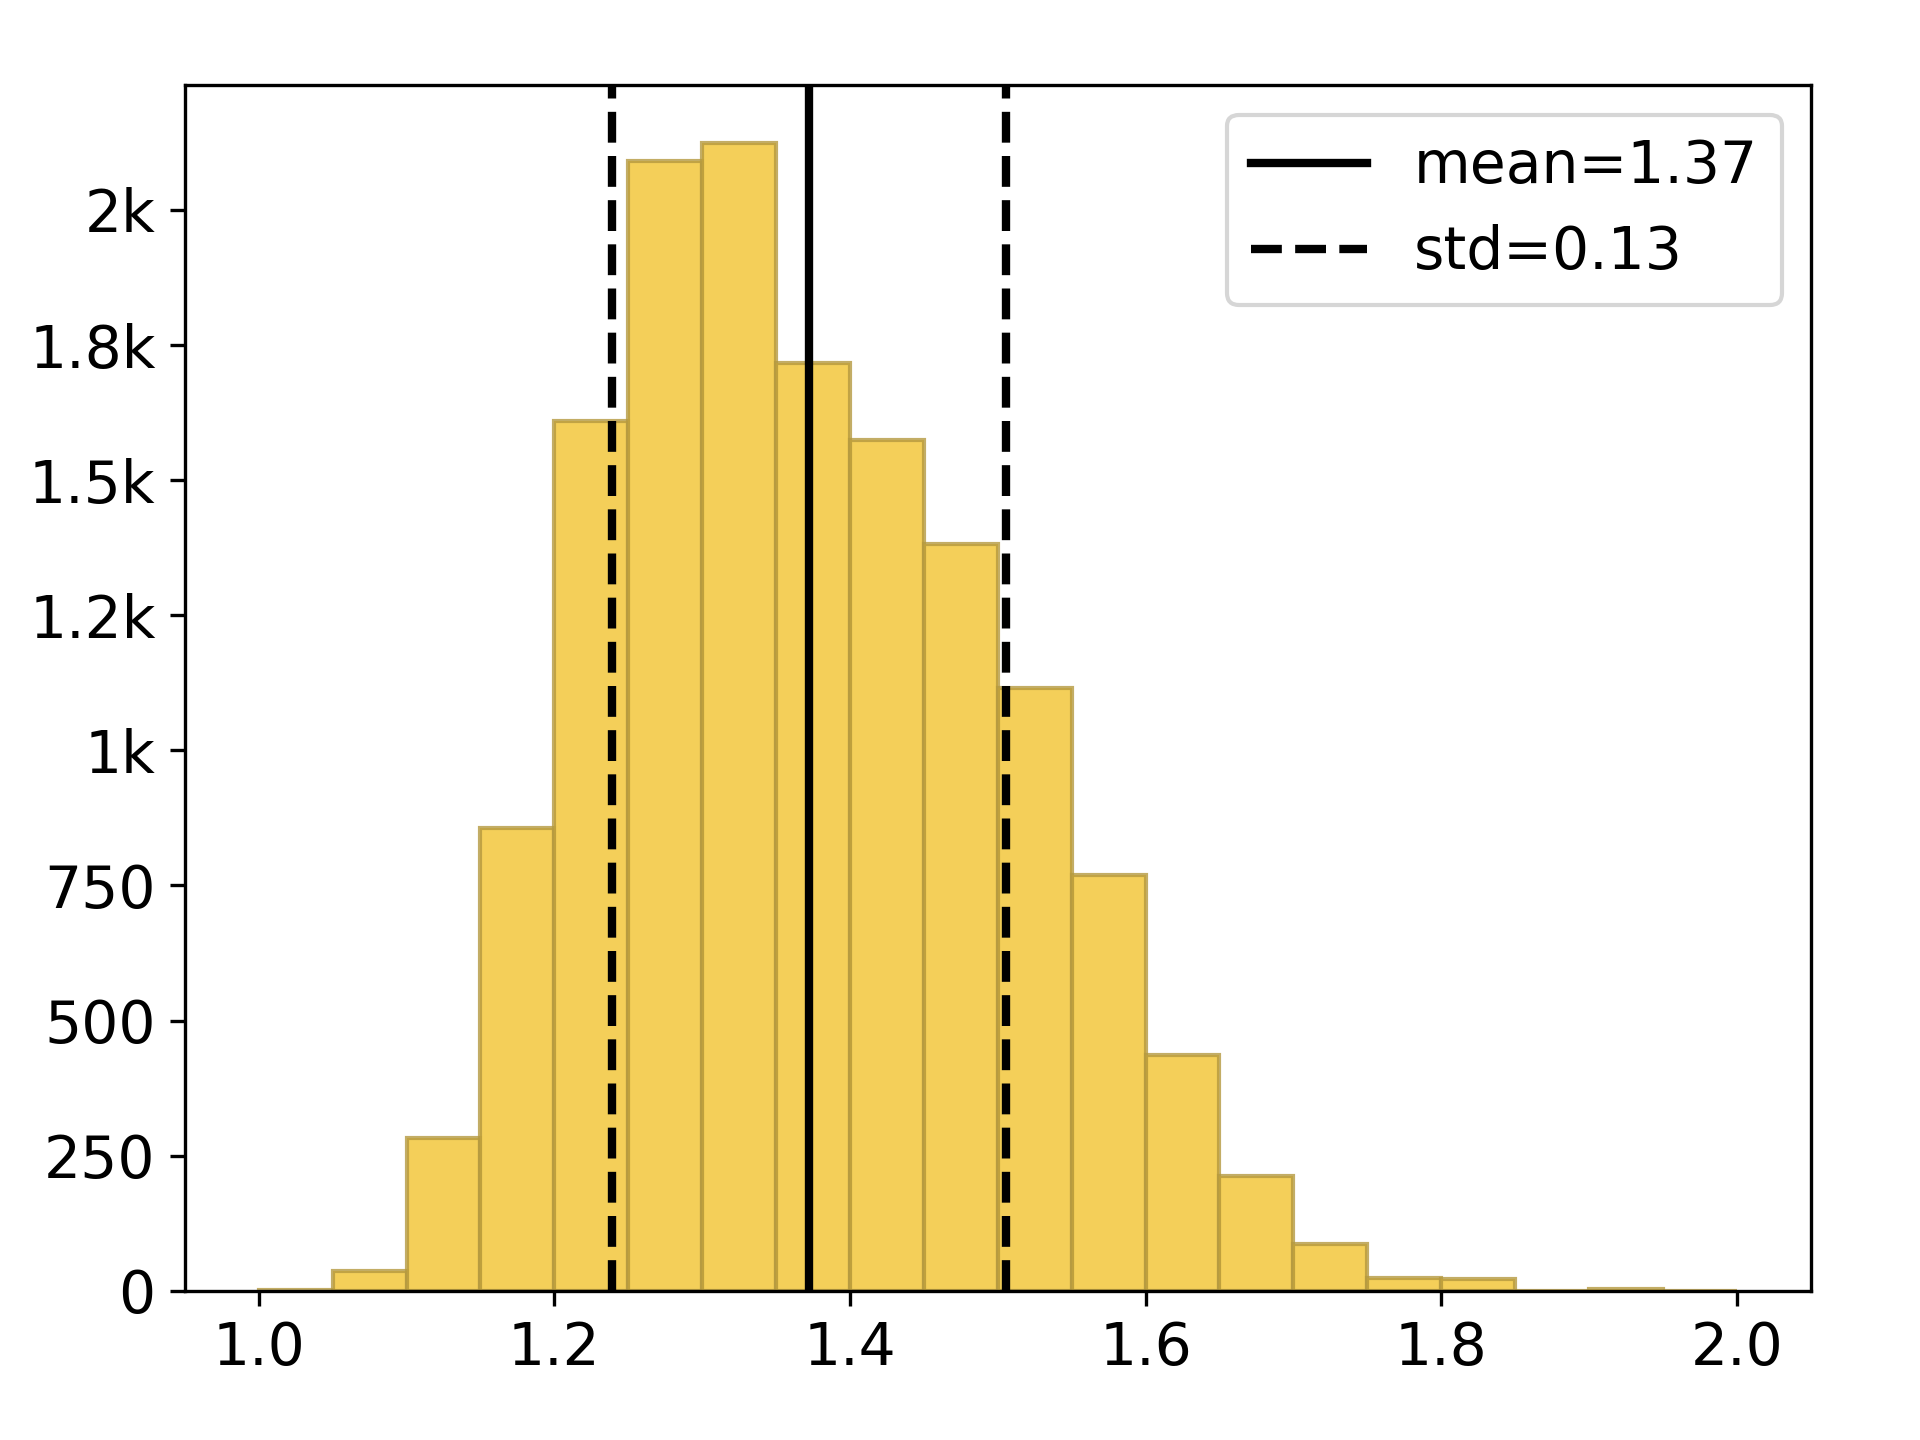
\includegraphics[width=\textwidth, clip,, trim=.25cm 0.25cm .25cm 0.25cm]{Resources/Images/Histogram/hist_1_a.png}
	\end{minipage}
	\begin{minipage}{.325\textwidth}
		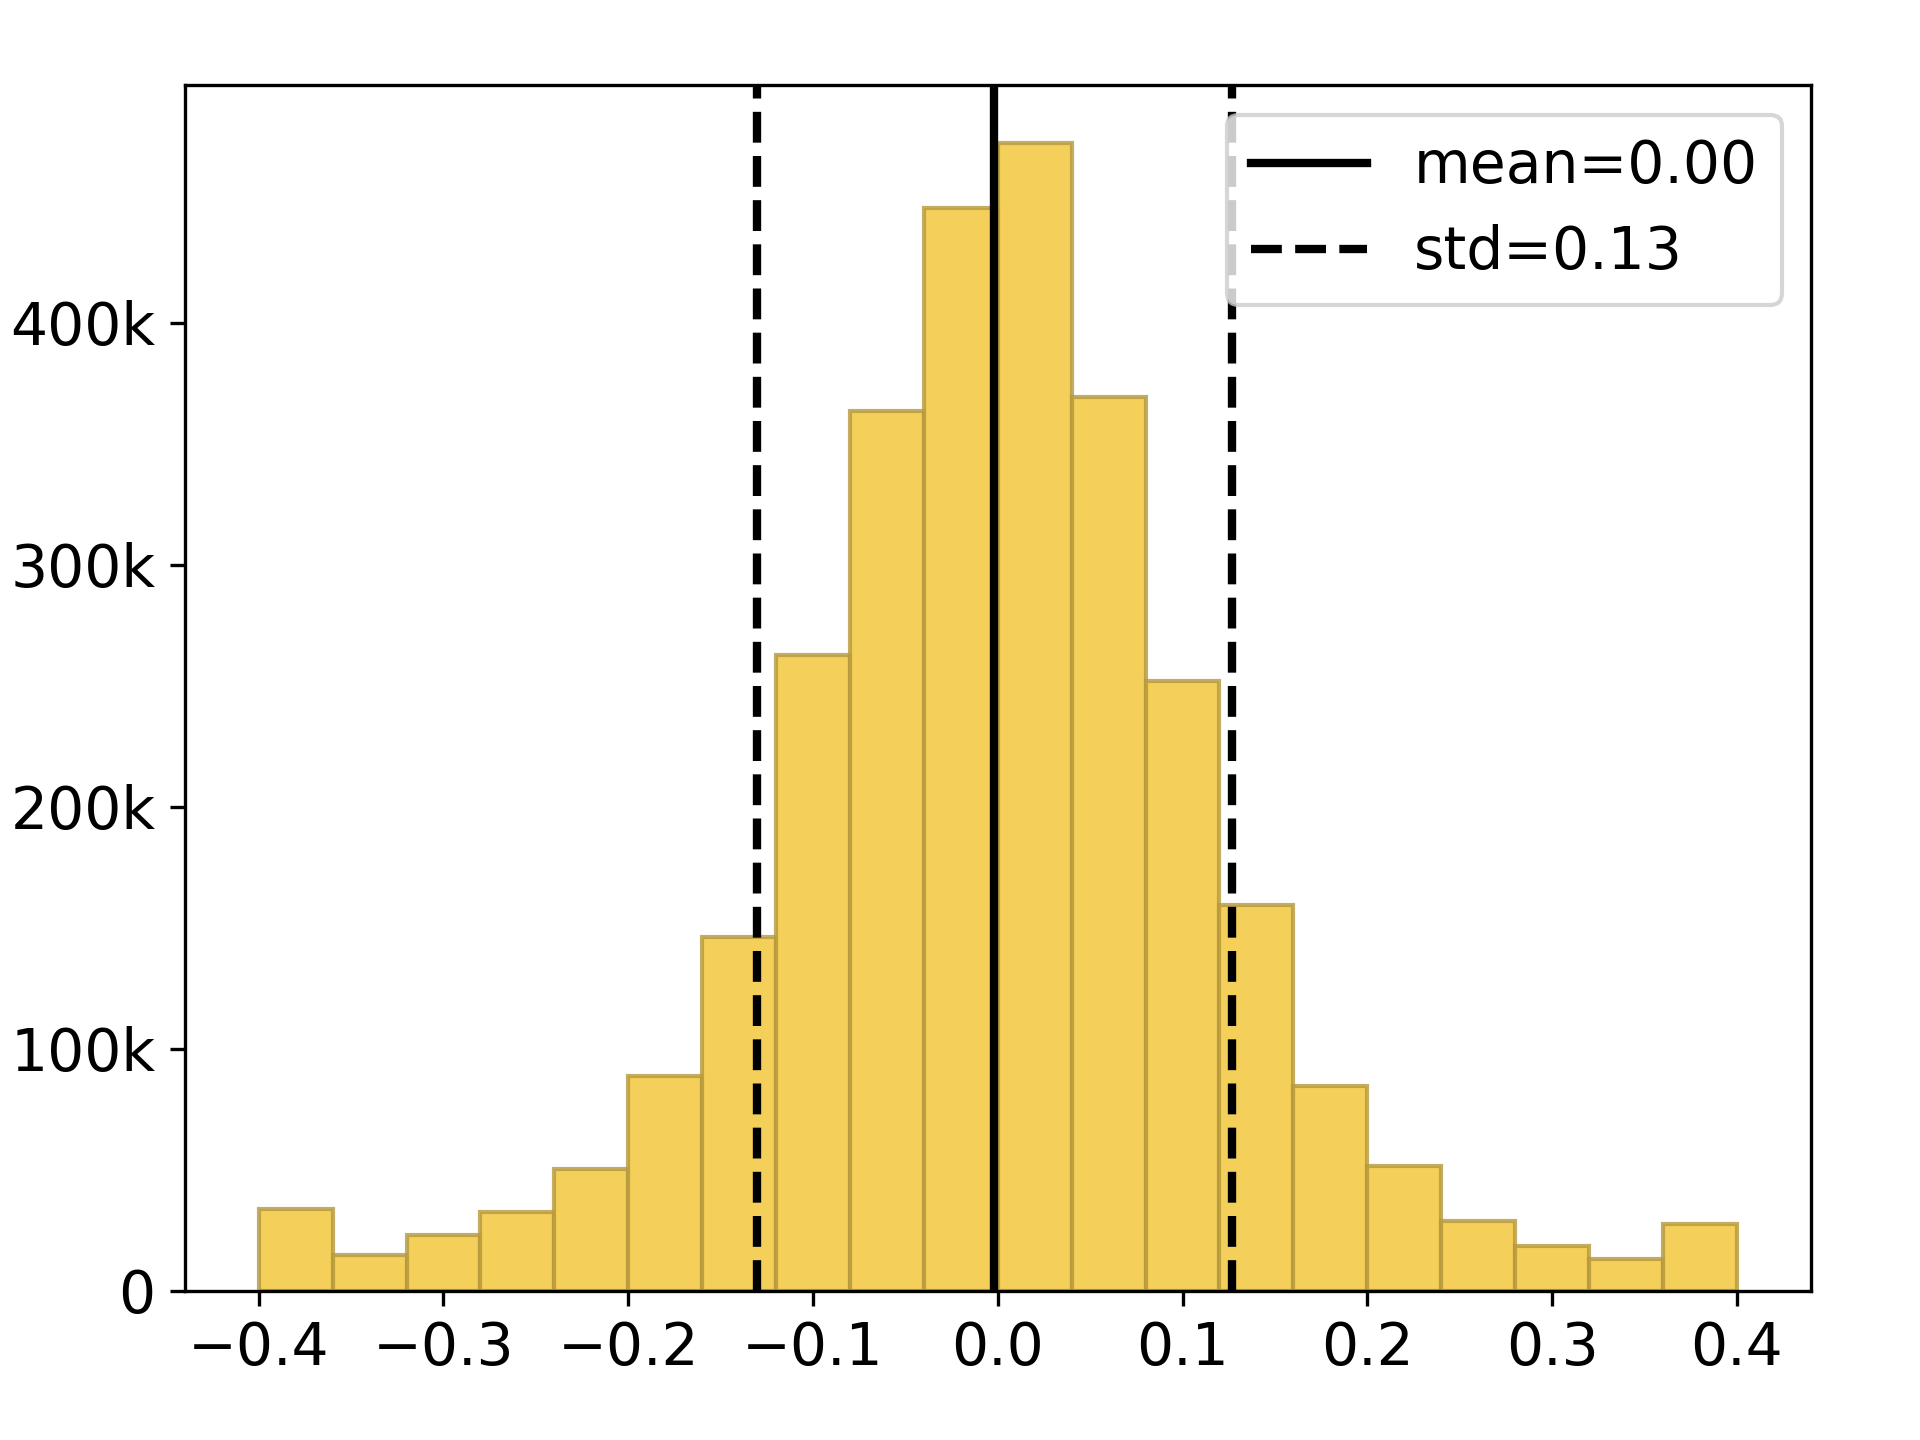
\includegraphics[width=\textwidth, clip, trim=.25cm 0.25cm .25cm 0.25cm]{Resources/Images/Histogram/hist_2_a.png}
	\end{minipage}
	\begin{minipage}{.325\textwidth}
		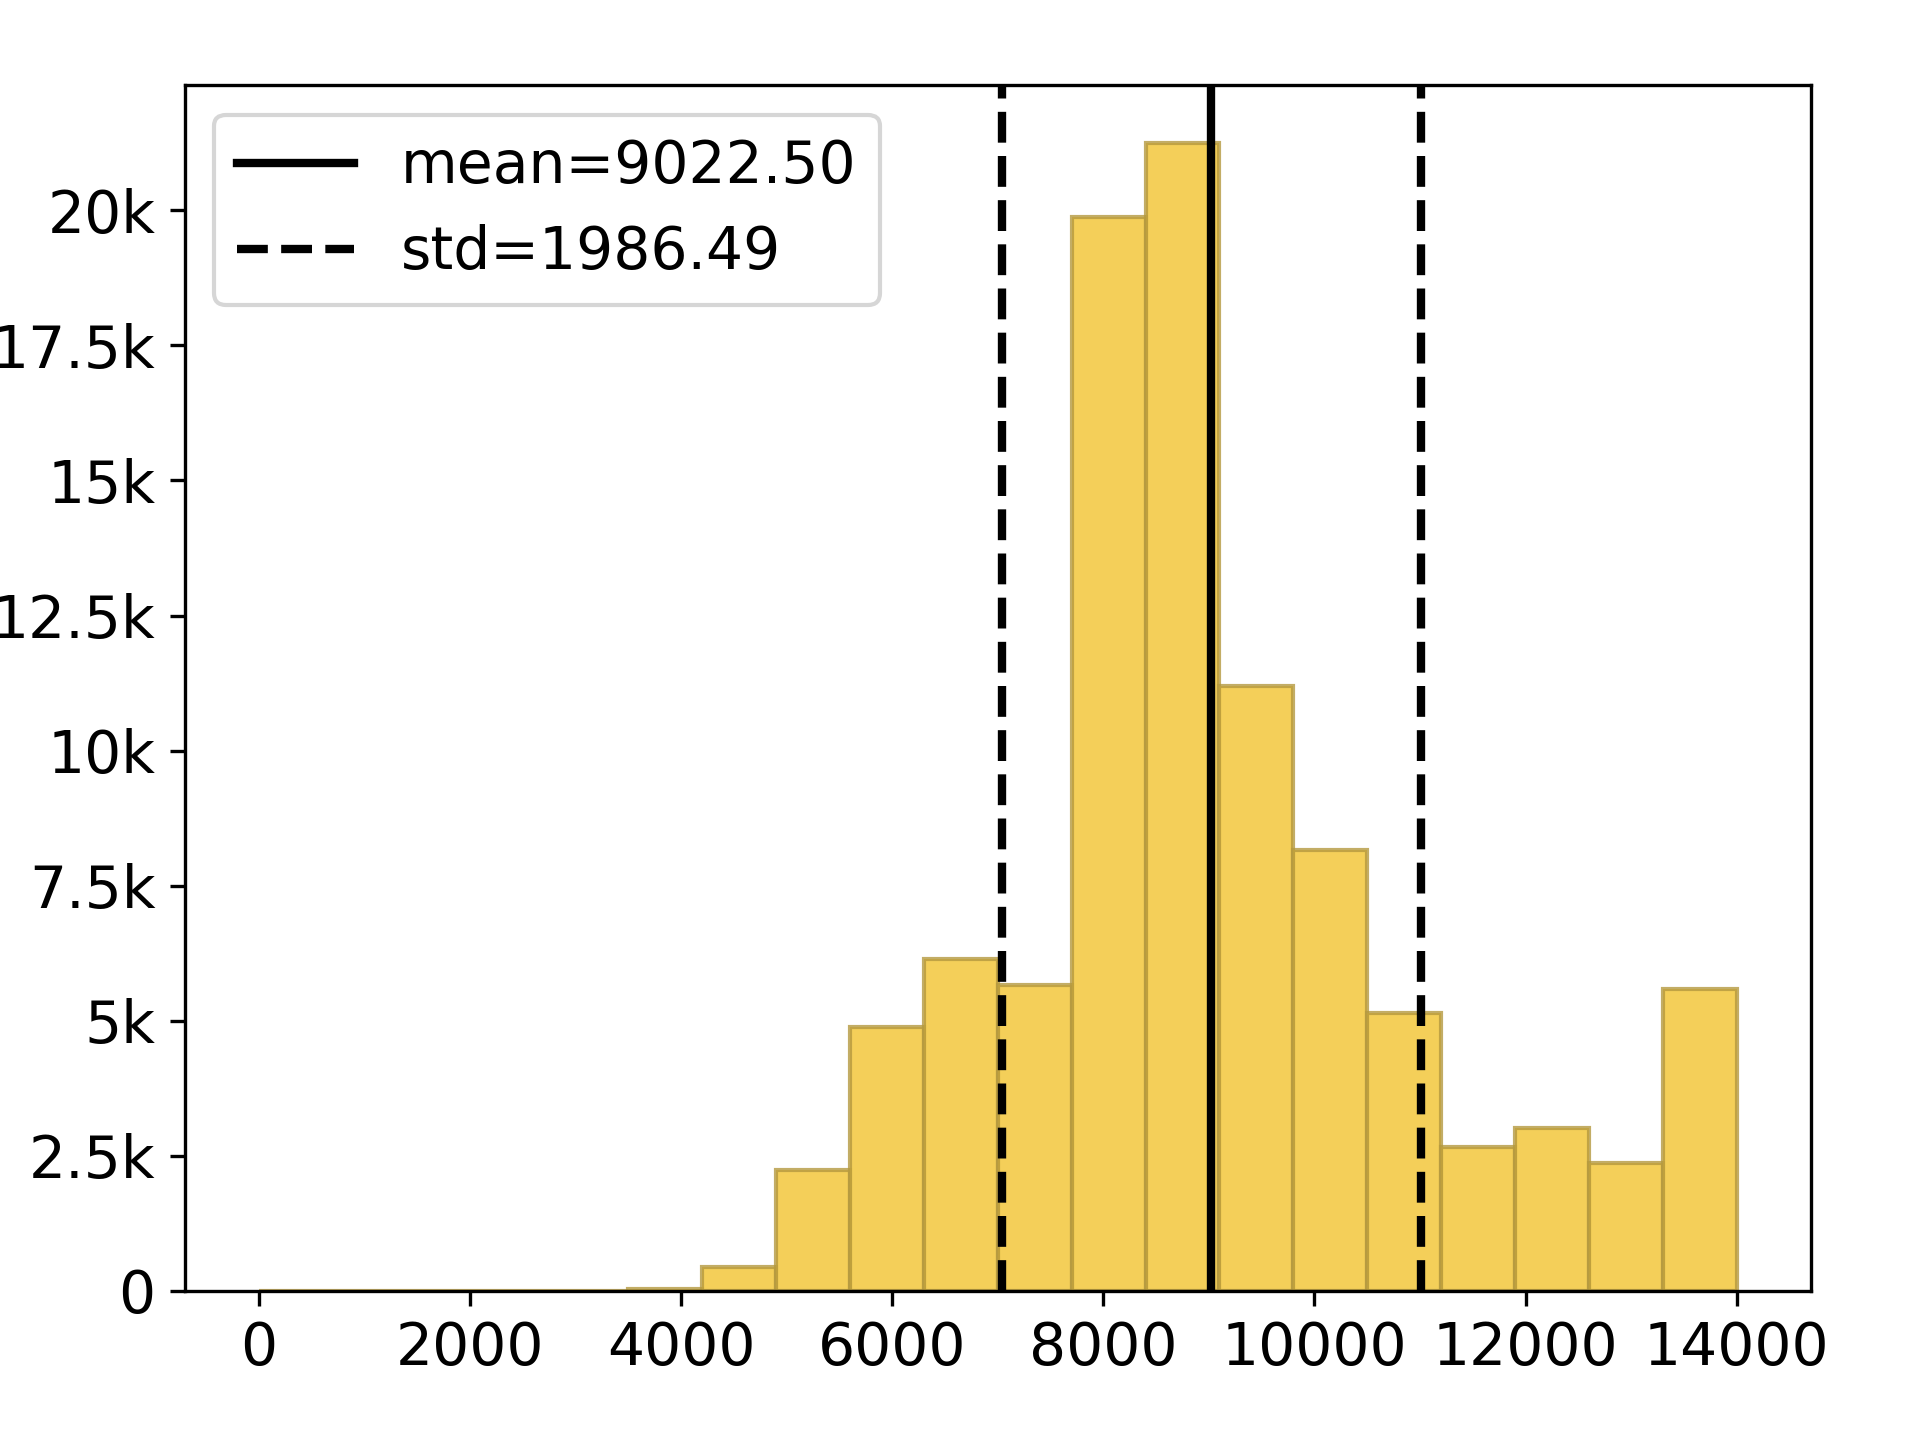
\includegraphics[width=\textwidth, clip, trim=.25cm 0.25cm .25cm 0.25cm]{Resources/Images/Histogram/hist_3_a.png}
	\end{minipage}
	
	\begin{minipage}{.325\textwidth}
		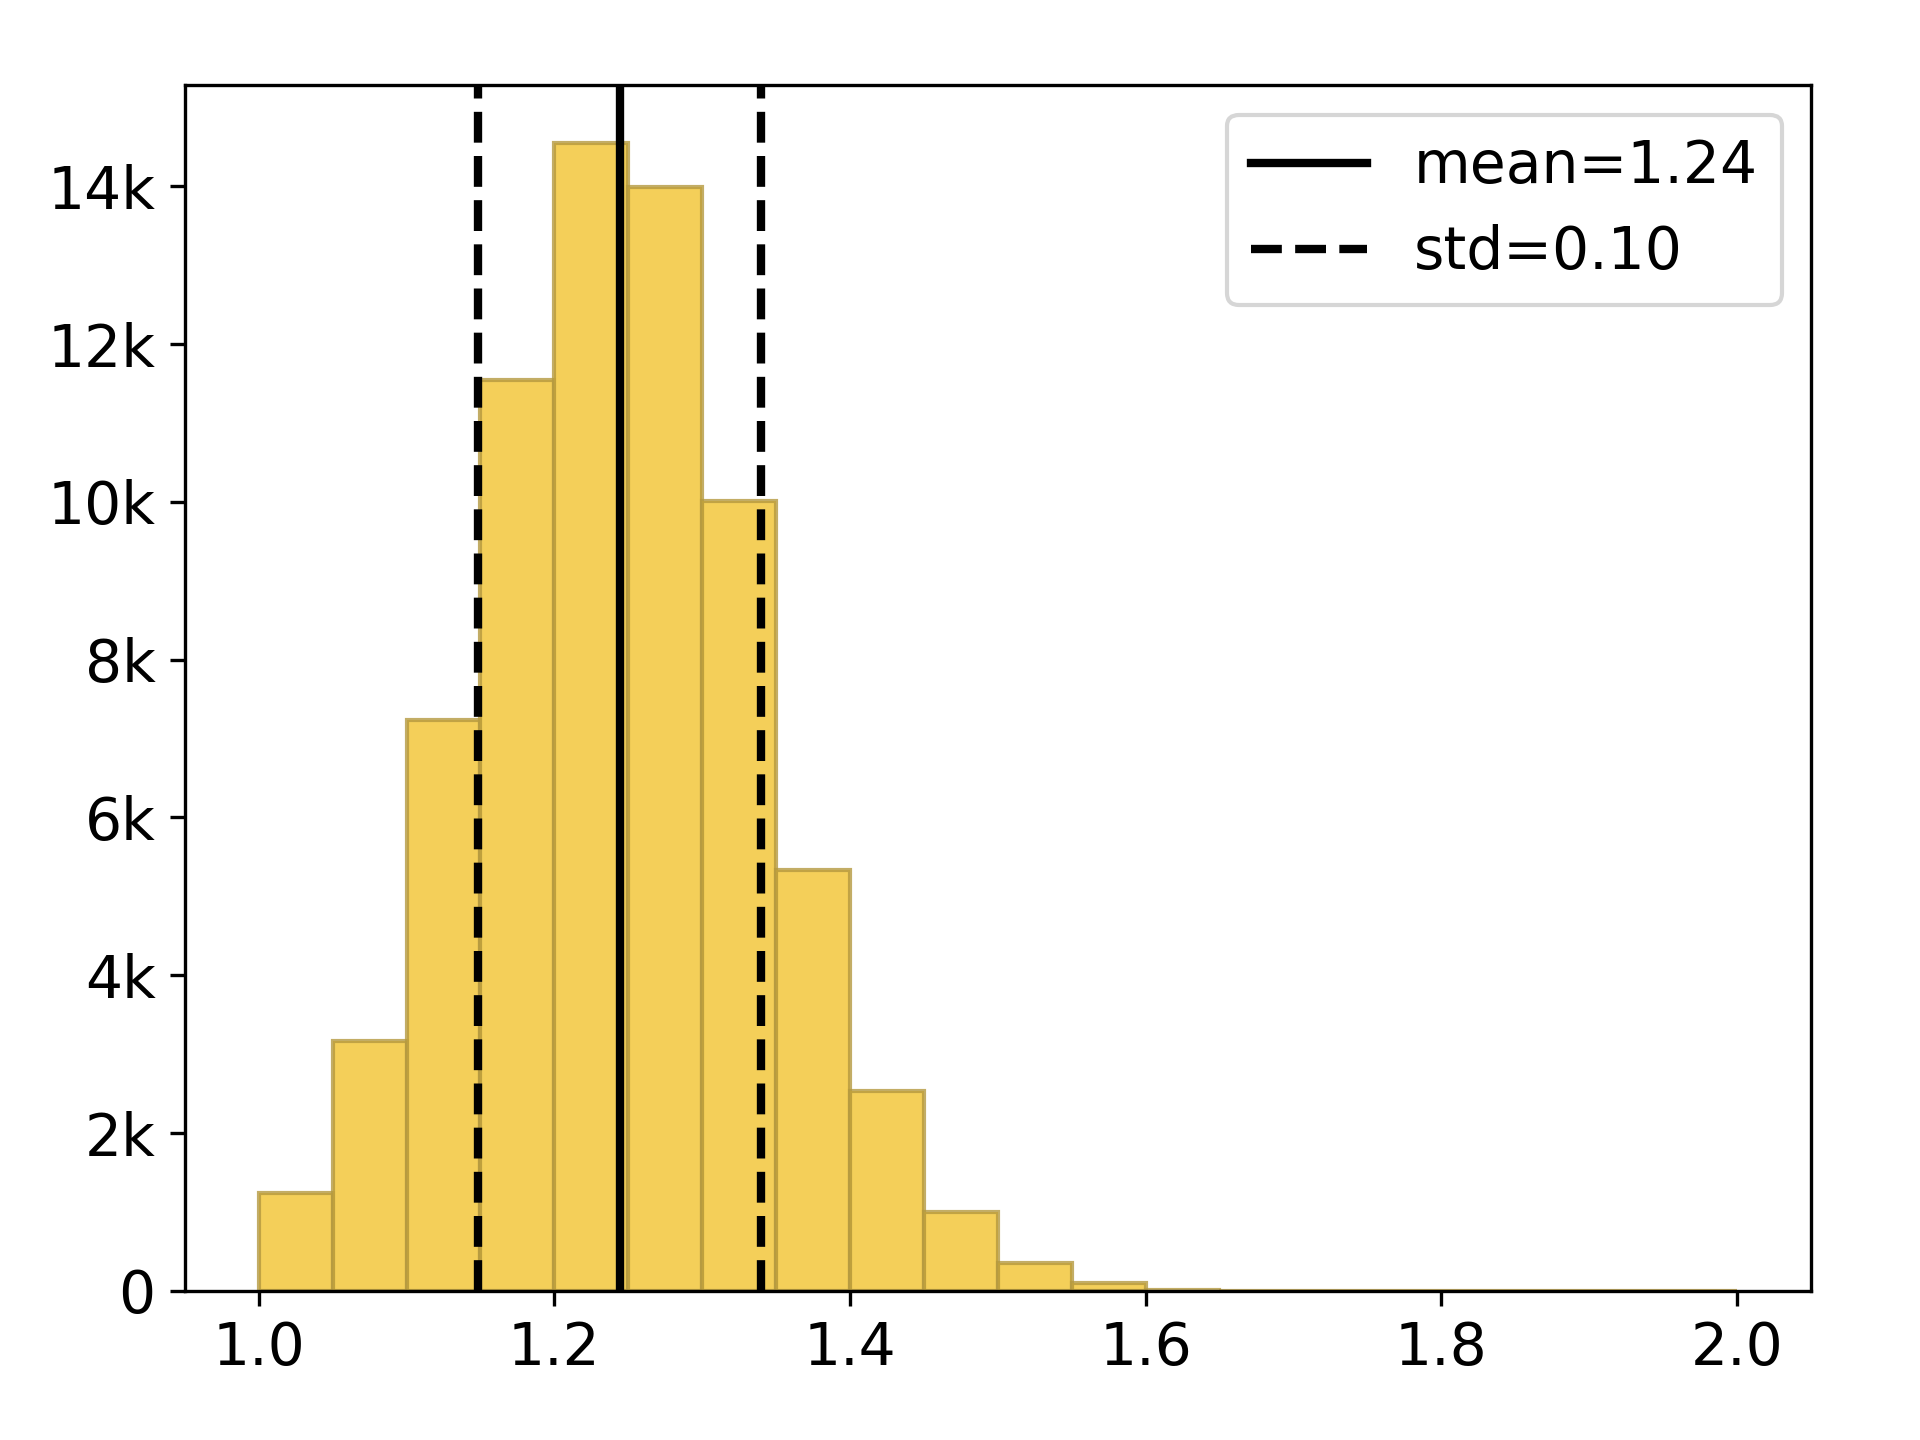
\includegraphics[width=\textwidth, trim=.25cm 0.25cm .25cm 0.25cm]{Resources/Images/Histogram/hist_1_b.png}
	\end{minipage}
	\begin{minipage}{.325\textwidth}
		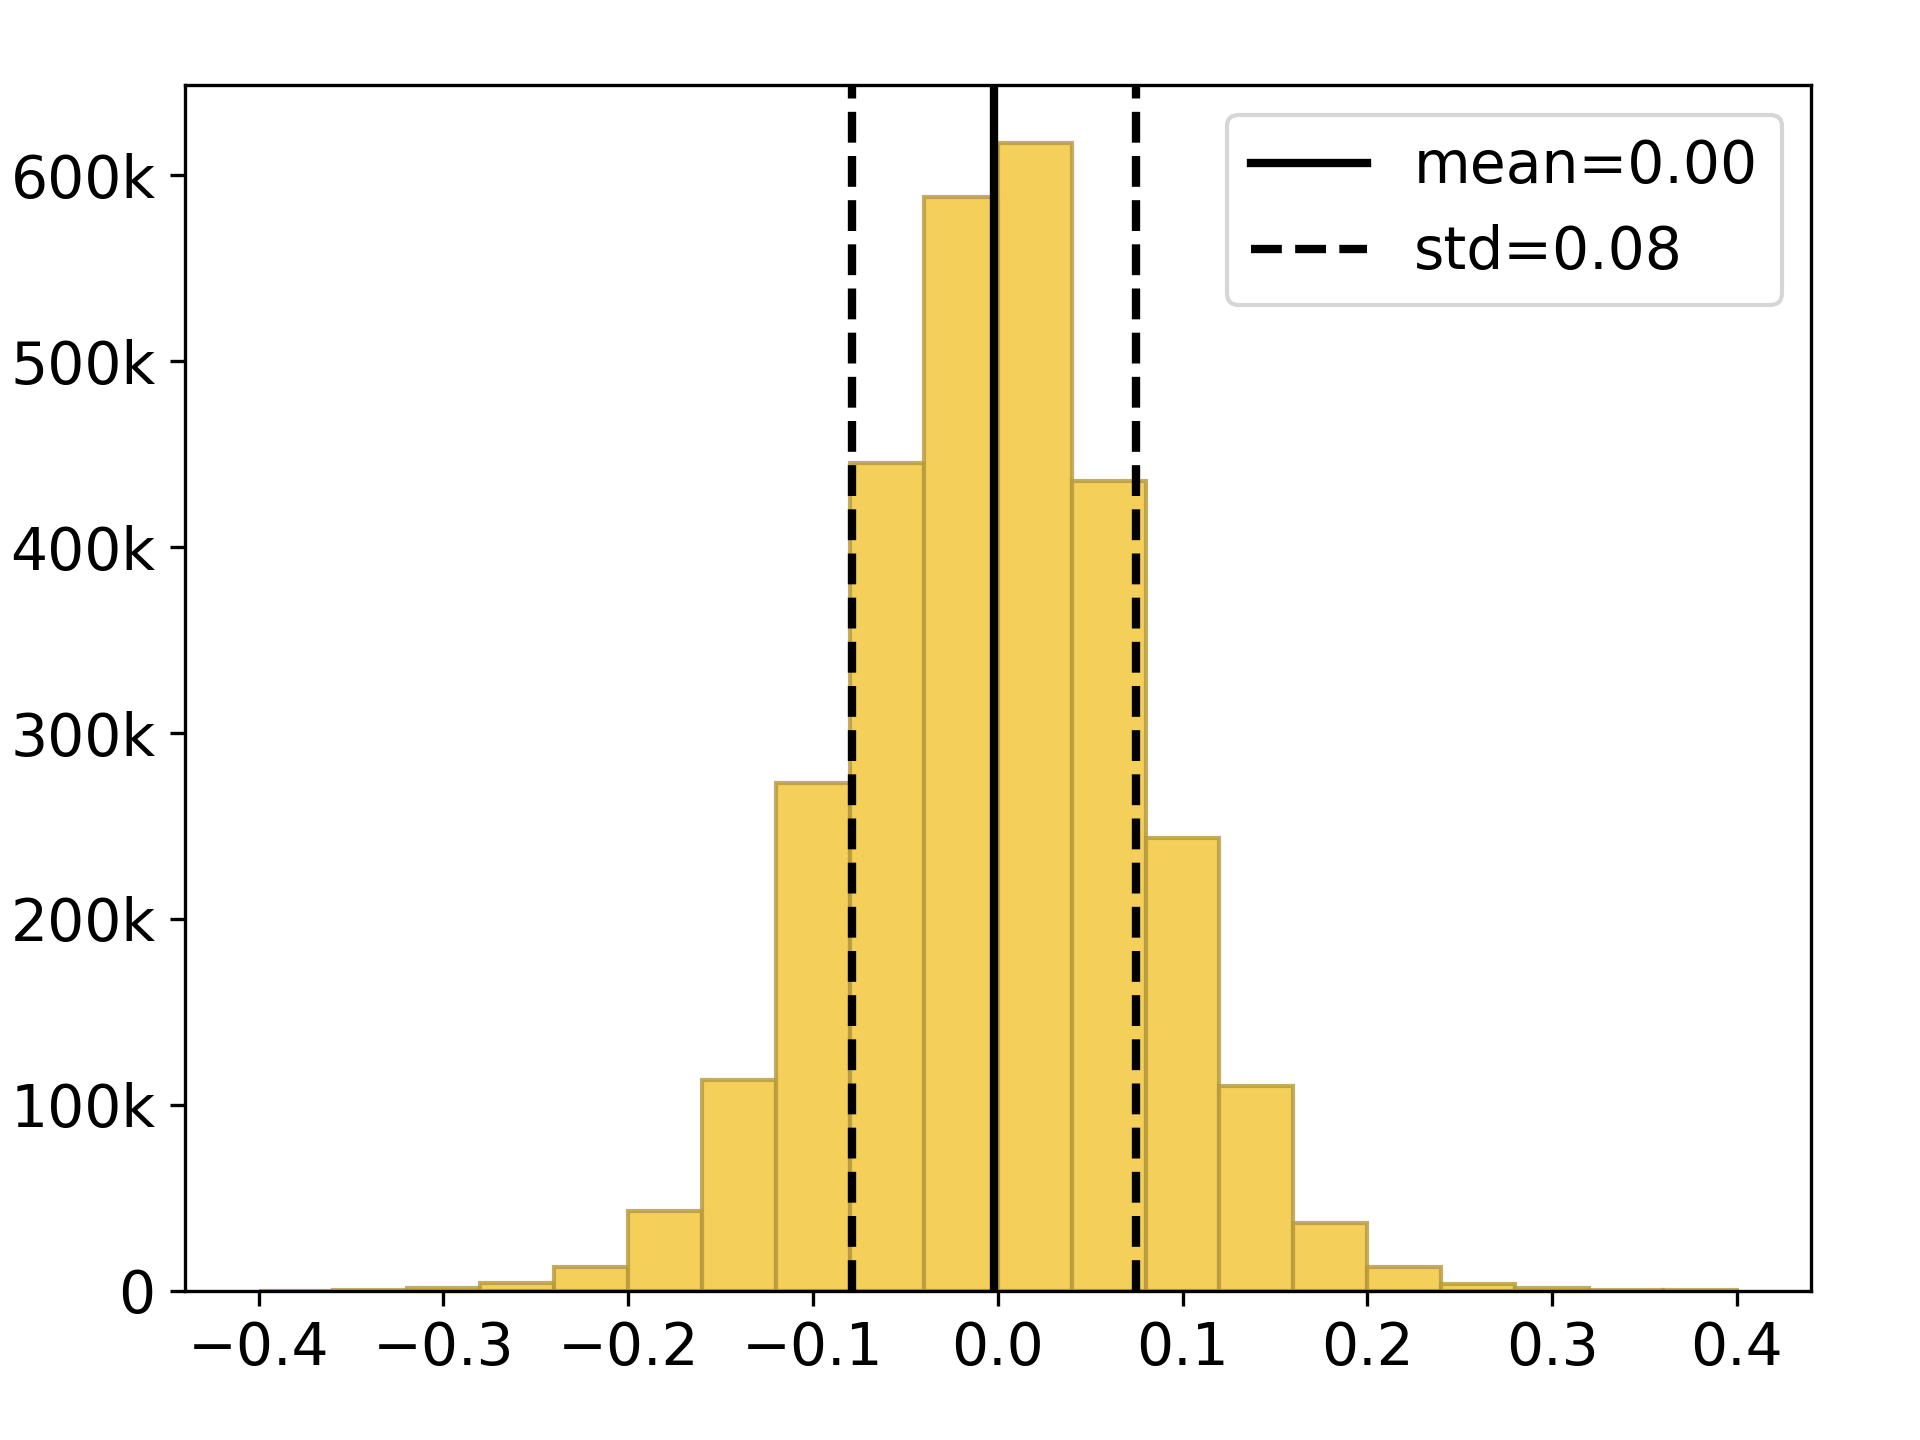
\includegraphics[width=\textwidth, clip, trim=.25cm 0.25cm .25cm 0.25cm]{Resources/Images/Histogram/hist_2_b.png}
	\end{minipage}
	\begin{minipage}{.325\textwidth}
		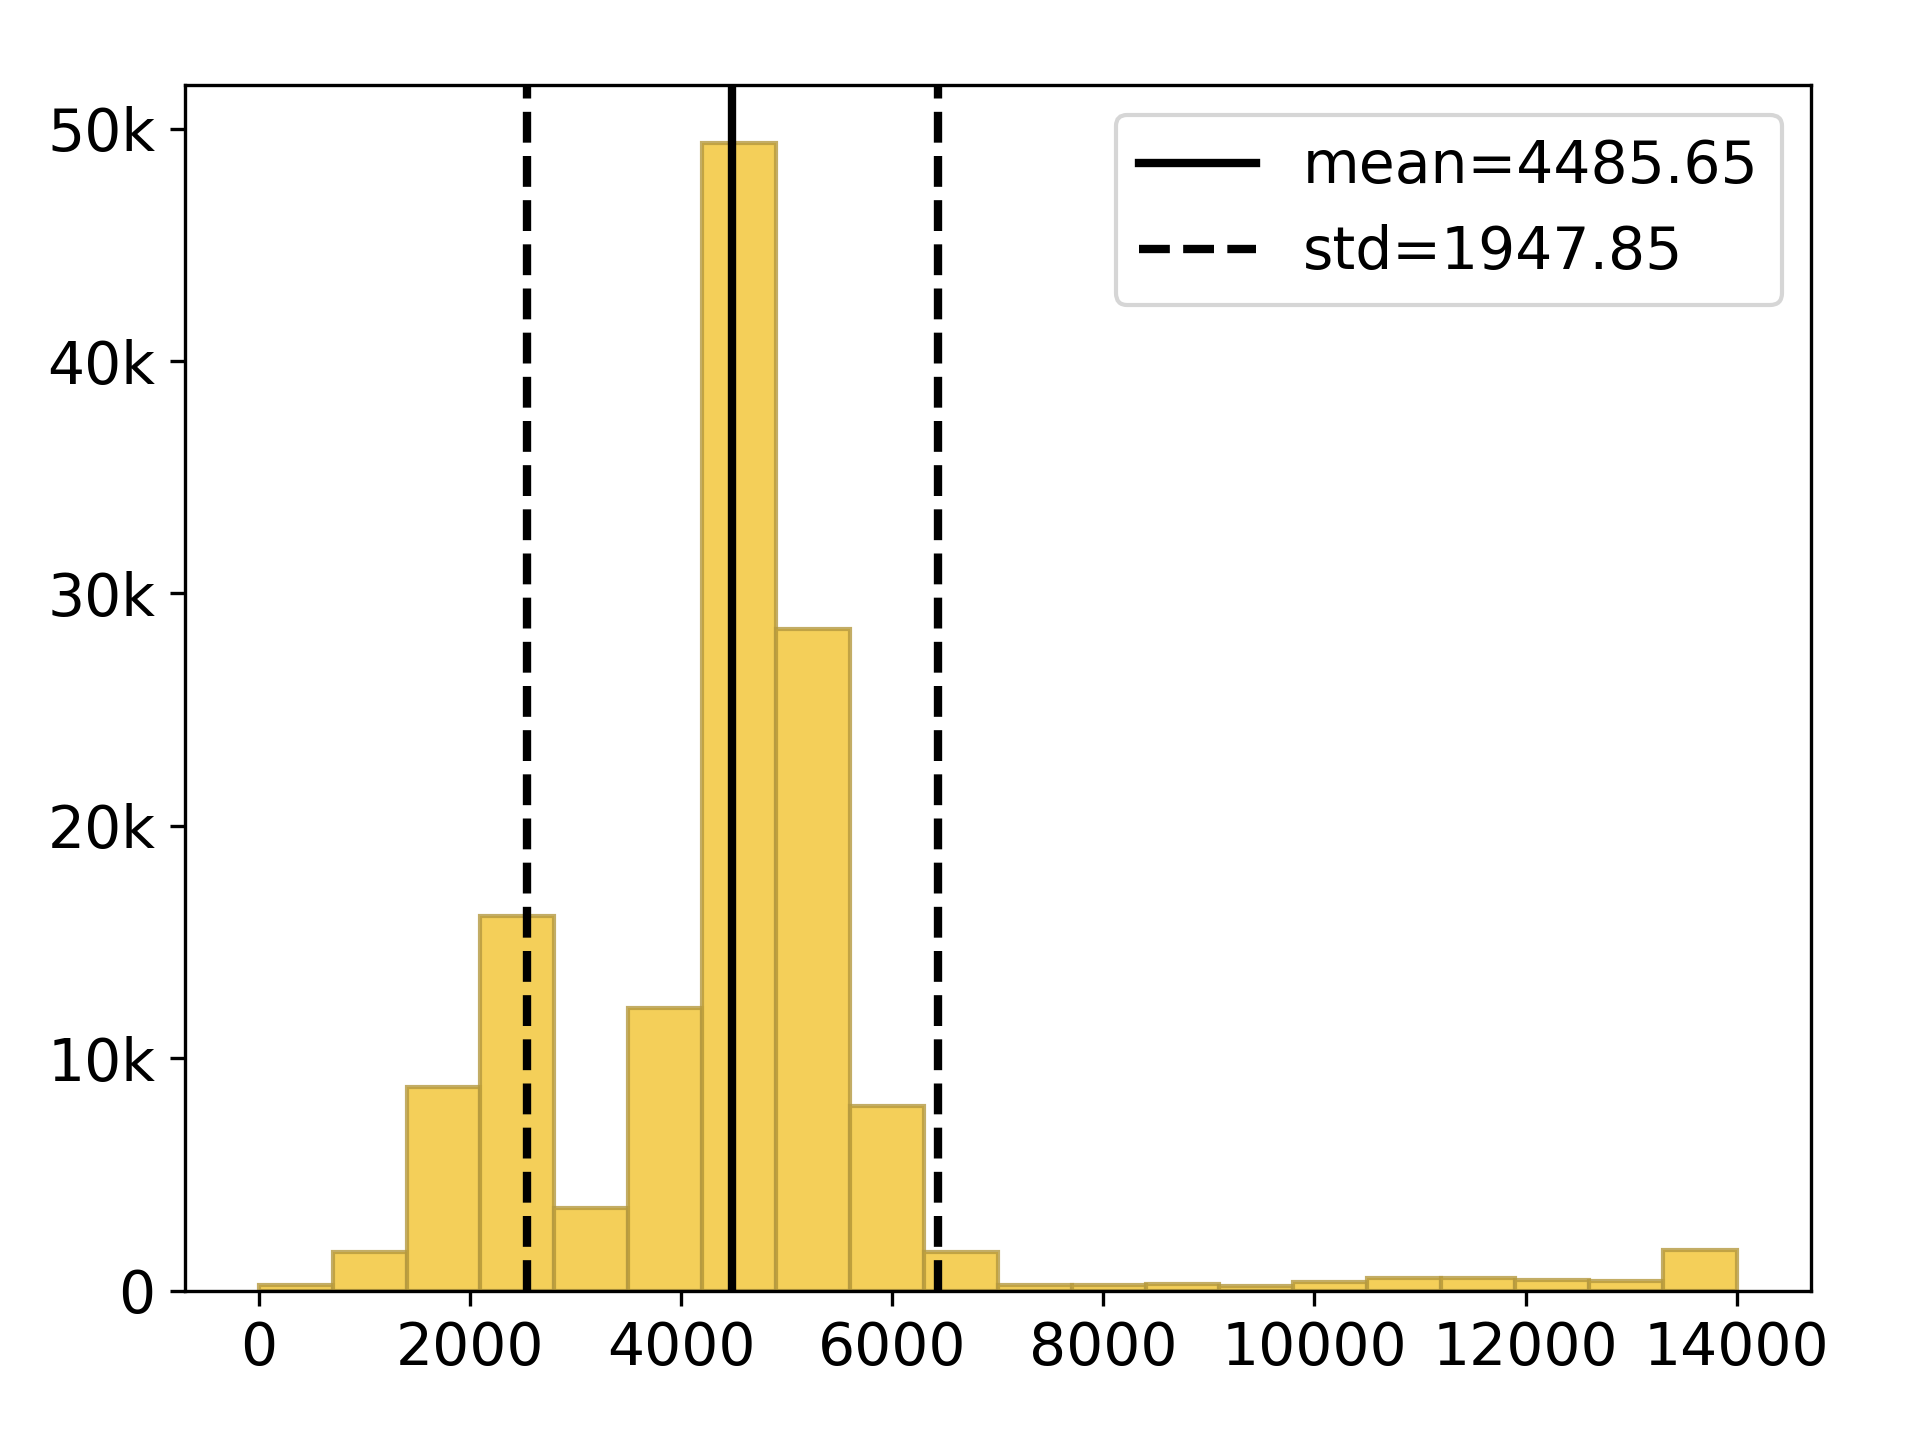
\includegraphics[width=\textwidth, trim=.25cm 0.25cm .25cm 0.25cm]{Resources/Images/Histogram/hist_3_b.png}
	\end{minipage}
	\caption{f.l.t.r. Histogram 1, Histogram 2, Histogram 3: Comparison of something (top row) and something different (bottom row)}
	\label{fig:images:histograms}
\end{figure}

	\section{Formulas}
\label{sec:formulas}

\begin{align}
	\textbf{AVG} ={}& \dfrac{1}{n} \, \sum_{i=1}^{n} \, a\textsubscript{i}
	\label{eq:formulas:average}
\end{align}

The average calculated per data window neglects all the past data windows and is relatively sensitive to outliers.
To make it more robust to temporary changes we can use the exponentially weighted moving average.
It is a combination of the current data window and the past data windows.
It weighs the current computed average by a factor $\alpha$ (e.g. 0.1) and all the past values combined by a factor 1 - $\alpha$ (e.g. 0.9).
It never really \textit{forgets} about the past, but weighs past values exponentially less with each step.

\begin{align}
    \textbf{EWMA($\alpha$)\textsubscript{t}} = 
	\begin{cases} 
		\ \mbox{AVG}\textsubscript{t}, & \mbox{if } t\mbox{ = 1} \\ 
		\ \alpha * \mbox{AVG}\textsubscript{t} + (1 - \alpha) * \mbox{AVG}\textsubscript{t-1} , & \mbox{if } t\mbox{ $>$ 1}
	\end{cases}
	\label{eq:formulas:moving_average}
\end{align}

\begin{align}
	\textbf{MAD(X)} = median(\Bigl| \ \mbox{X\textsubscript{i}} - median(\mbox{X}) \ \Bigl|)
	\label{eq:formulas:mad}
\end{align}

\begin{align}
\begin{split}
    \textbf{P} ={}& number\,of\,positives\,in\,ground\,truth
\end{split}\\
\begin{split}
    \textbf{N} ={}& number\,of\,negatives\,in\,ground\,truth
\end{split}\\
\begin{split}
    \textbf{TP} ={}& number\,of\,true\,positives
\end{split}\\
\begin{split}
    \textbf{FP} ={}& number\,of\,false\,positives
\end{split}\\
\begin{split}
    \textbf{FN} ={}& number\,of\,false\,negatives
\end{split}\\[1ex]
\begin{split}
    \textbf{recall} ={}& \frac{TP}{TP+FN} \label{eq:results:recall}
\end{split}\\[1ex]
\begin{split}
    \textbf{precision} ={}& \frac{TP}{TP+FP} \label{eq:formulas:precision}
\end{split}\\[1ex]
\begin{split}
    \textbf{F1 score} ={}& 2 * \frac{precision * recall}{precision + recall} \label{eq:formulas:f1}
\end{split}\\[1ex]
\begin{split}
    \textbf{accuracy} ={}& \frac{TP+TN}{P+N} \label{eq:formulas:accuracy}
\end{split}
\end{align}


	\section{Conclusion}
\label{sec:conclusion}

Lorem ipsum dolor sit amet, consetetur sadipscing elitr, sed diam nonumy eirmod tempor invidunt ut labore et dolore magna aliquyam erat, sed diam voluptua. At vero eos et accusam et justo duo dolores et ea rebum. Stet clita kasd gubergren, no sea takimata sanctus est Lorem ipsum dolor sit amet. Lorem ipsum dolor sit amet, consetetur sadipscing elitr, sed diam nonumy eirmod tempor invidunt ut labore et dolore magna aliquyam erat, sed diam voluptua. At vero eos et accusam et justo duo dolores et ea rebum. Stet clita kasd gubergren, no sea takimata sanctus est Lorem ipsum dolor sit amet. Lorem ipsum dolor sit amet, consetetur sadipscing elitr, sed diam nonumy eirmod tempor invidunt ut labore et dolore magna aliquyam erat, sed diam voluptua. At vero eos et accusam et justo duo dolores et ea rebum. Stet clita kasd gubergren, no sea takimata sanctus est Lorem ipsum dolor sit amet.   

Duis autem vel eum iriure dolor in hendrerit in vulputate velit esse molestie consequat, vel illum dolore eu feugiat nulla facilisis at vero eros et accumsan et iusto odio dignissim qui blandit praesent luptatum zzril delenit augue duis dolore te feugait nulla facilisi. Lorem ipsum dolor sit amet, consectetuer adipiscing elit, sed diam nonummy nibh euismod tincidunt ut laoreet dolore magna aliquam erat volutpat.   

Ut wisi enim ad minim veniam, quis nostrud exerci tation ullamcorper suscipit lobortis nisl ut aliquip ex ea commodo consequat. Duis autem vel eum iriure dolor in hendrerit in vulputate velit esse molestie consequat, vel illum dolore eu feugiat nulla facilisis at vero eros et accumsan et iusto odio dignissim qui blandit praesent luptatum zzril delenit augue duis dolore te feugait nulla facilisi.   

Nam liber tempor cum soluta nobis eleifend option congue nihil imperdiet doming id quod mazim placerat facer possim assum. Lorem ipsum dolor sit amet, consectetuer adipiscing elit, sed diam nonummy nibh euismod tincidunt ut laoreet dolore magna aliquam erat volutpat. Ut wisi enim ad minim veniam, quis nostrud exerci tation ullamcorper suscipit lobortis nisl ut aliquip ex ea commodo consequat.   

Duis autem vel eum iriure dolor in hendrerit in vulputate velit esse molestie consequat, vel illum dolore eu feugiat nulla facilisis.   

At vero eos et accusam et justo duo dolores et ea rebum. Stet clita kasd gubergren, no sea takimata sanctus est Lorem ipsum dolor sit amet. Lorem ipsum dolor sit amet, consetetur sadipscing elitr, sed diam nonumy eirmod tempor invidunt ut labore et dolore magna aliquyam erat, sed diam voluptua.
	\printglossary
	\newpage
	\bibliography{quotations}
	\newpage
	\listoffigures
	\newpage
	\listoftables
	\newpage
	\phantomsection %needed that toc links work
	\addcontentsline{toc}{section}{Declaration of Academic Integrity}
	\section*{Declaration of Academic Integrity}
\label{sec:authenticity_agreement}

Hereby, I declare that I have composed the presented paper independently on my own and without any other resources than the ones indicated. All thoughts taken directly or indirectly from external sources are properly denoted as such. This paper has neither been previously submitted to another authority nor has it been published yet.

\vspace{1cm}

\noindent\begin{tabular}{@{}ll}
	Zurich, 01.01.1970 & 
\includegraphics[width=4cm]{Resources/Images/AuthenticityAgreement/signature} \\[-1.5ex]
	\makebox[6cm]{\hrulefill} & \makebox[6cm]{\hrulefill}\\ 
	Location, date & Signature John Doe\\
\end{tabular}

	\phantomsection %needed that toc links work
	\addcontentsline{toc}{section}{Appendix}
	\section*{Appendix}
\label{sec:appendix}

Lorem ipsum dolor sit amet, consetetur sadipscing elitr, sed diam nonumy eirmod tempor invidunt ut labore et dolore magna aliquyam erat, sed diam voluptua. At vero eos et accusam et justo duo dolores et ea rebum. Stet clita kasd gubergren, no sea takimata sanctus est Lorem ipsum dolor sit amet. Lorem ipsum dolor sit amet, consetetur sadipscing elitr, sed diam nonumy eirmod tempor invidunt ut labore et dolore magna aliquyam erat, sed diam voluptua. At vero eos et accusam et justo duo dolores et ea rebum. Stet clita kasd gubergren, no sea takimata sanctus est Lorem ipsum dolor sit amet. Lorem ipsum dolor sit amet, consetetur sadipscing elitr, sed diam nonumy eirmod tempor invidunt ut labore et dolore magna aliquyam erat, sed diam voluptua. At vero eos et accusam et justo duo dolores et ea rebum. Stet clita kasd gubergren, no sea takimata sanctus est Lorem ipsum dolor sit amet.

Duis autem vel eum iriure dolor in hendrerit in vulputate velit esse molestie consequat, vel illum dolore eu feugiat nulla facilisis at vero eros et accumsan et iusto odio dignissim qui blandit praesent luptatum zzril delenit augue duis dolore te feugait nulla facilisi. Lorem ipsum dolor sit amet, consectetuer adipiscing elit, sed diam nonummy nibh euismod tincidunt ut laoreet dolore magna aliquam erat volutpat.

Ut wisi enim ad minim veniam, quis nostrud exerci tation ullamcorper suscipit lobortis nisl ut aliquip ex ea commodo consequat. Duis autem vel eum iriure dolor in hendrerit in vulputate velit esse molestie consequat, vel illum dolore eu feugiat nulla facilisis at vero eros et accumsan et iusto odio dignissim qui blandit praesent luptatum zzril delenit augue duis dolore te feugait nulla facilisi.

Nam liber tempor cum soluta nobis eleifend option congue nihil imperdiet doming id quod mazim placerat facer possim assum. Lorem ipsum dolor sit amet, consectetuer adipiscing elit, sed diam nonummy nibh euismod tincidunt ut laoreet dolore magna aliquam erat volutpat. Ut wisi enim ad minim veniam, quis nostrud exerci tation ullamcorper suscipit lobortis nisl ut aliquip ex ea commodo consequat.

Duis autem vel eum iriure dolor in hendrerit in vulputate velit esse molestie consequat, vel illum dolore eu feugiat nulla facilisis.

At vero eos et accusam et justo duo dolores et ea rebum. Stet clita kasd gubergren, no sea takimata sanctus est Lorem ipsum dolor sit amet. Lorem ipsum dolor sit amet, consetetur

	
\end{document}
